\section{Introduction}
\label{chap2-sec:intro}
Counting subgraphs (e.g., triangles, stars, cycles) is
% a fundamental task 
one of the most basic tasks 
for analyzing connection patterns
% for analyzing graph statistics
in
% a graph.
various graph data, e.g., social,
communication, and collaboration networks.
% , epidemiological networks.
% Graph statistics is important to understand the connection patterns in various graph data; e.g., social networks, collaboration networks,
% For example, a degree distribution in a social graph represents a distribution of the number of friends in the graph.
% A subgraph count (e.g.,
For example,
% a triangle count is the number of three nodes with three edges.
% A $k$-star count is the number of a node connected to $k$ other nodes.
a triangle is given by a set of three nodes with three edges, whereas a $k$-star is given by a central node connected to $k$ other nodes.
% a set of $k$ nodes connected a central node.
These subgraphs
% are important because they can be used to calculate
play a crucial role in calculating
a \textit{clustering coefficient} ($=\frac{3 \times \text{\#triangles}}{\text{\#2-stars}}$) (see Figure~\ref{chap2-fig:triangles_stars}). 
% which 
The clustering coefficient 
measures the average probability that
two friends of a user will also be a friend
% a friend's friend is also a friend
in a social graph \cite{Newman_PRL09}. 
Therefore, it is useful for measuring the effectiveness of friend suggestions. 
In addition, the clustering coefficient represents the degree to which users tend to cluster together. 
Thus, if it is large in some services/communities, we can effectively apply social recommendations \cite{Kolluri_CCS21} to the users. 
% for an example of
% the triangle and $k$-star counts and clustering coefficient).
% these subgraph counts).
% \cite{Newman_PRL09}.
% It is also known that these subgraphs are sufficient statistics for exponential random graph models
Triangles 
and $k$-stars 
% can also be used for
are also useful for 
% modeling graphs \cite{Jorgensen_SIGMOD16,Robins_SN07}.
% generating graphs based on some
constructing
graph models
\cite{Robins_SN07,Jorgensen_SIGMOD16}; 
% and other applications \cite{Imola_USENIX21}.
% (e.g., exponential random graph models \cite{Robins_SN07}, TriCycle \cite{Jorgensen_SIGMOD16}).
% Applications of triangle counting are summarized in \cite{Tsourakakis_JGAA11}. 
see also \cite{Tsourakakis_JGAA11} for other applications of triangle counting. 
However, graph data often involve sensitive data such as sensitive edges (friendships),
% that a user wants to keep secret,
% which 
and they 
can be leaked from 
% exact values of triangle counts and $k$-star counts \cite{Imola_USENIX21}.
exact numbers of triangles and $k$-stars \cite{Imola_USENIX21}.
% Therefore,
% there is a need for
% we need to develop an algorithm for
% counting
% subgraphs while strongly protecting user privacy.
% , which is the focus of this paper.


To analyze subgraphs while protecting user privacy, DP (Differential Privacy) \cite{DP} has been widely adopted as a privacy metric \cite{Ding_TKDE21,Imola_USENIX21,Karwa_PVLDB11,Sun_CCS19,Ye_ICDE20,Ye_TKDE21,Zhang_SIGMOD15}.
DP protects user privacy against adversaries with arbitrary background knowledge and is known as a gold standard for data privacy.
% Most studies on private graph analysis \cite{Chen_PoPETs20,Day_SIGMOD16,Hay_ICDM09,Karwa_PVLDB11,Kasiviswanathan_TCC13,Nissim_STOC07,Raskhodnikova_arXiv15,Song_arXiv18} assumes central DP
According to the underlying model, DP can be categorized into \textit{central (or global) DP} and \textit{LDP (Local DP)}.
Central DP assumes a scenario where
% that
a central server has personal data of all users.
% whereas LDP does not assume such trusted servers.
Although accurate analysis of subgraphs is possible under
% central DP
this model \cite{Ding_TKDE21,Karwa_PVLDB11,Zhang_SIGMOD15}, there is a risk that the entire graph is leaked from the server by illegal access or internal fraud \cite{data_breach2021,CambridgeAnalytica}.
In addition, central DP cannot be applied to  \textit{decentralized social networks} 
\cite{Diaspora,Mastodon,Minds,Paul_CN14} 
% \cite{Diaspora,Mastodon,Paul_CN14} 
% (e.g., Diaspora \cite{Diaspora}, Mastodon \cite{Mastodon}) 
% which has no central server that has the entire graph, and uses many servers each of which has personal data of users who have registered
where the entire graph is distributed across many servers. 
% nor 
We can even consider 
\textit{fully decentralized applications} where a server does not have
any original edge, 
% between users, 
% information about the original edges;
% For example,
% mobile application in which each user sends the number of her friends
e.g., a mobile app that sends a noisy degree (noisy number of friends) to the server, which then estimates a degree distribution. 
Central DP cannot be used in such applications. 

In contrast, LDP assumes a scenario where each user obfuscates her personal data (friends list in 
the case of graphs) 
% data) 
by herself and sends the obfuscated data to a possibly malicious server; i.e., it does not assume trusted servers.
Thus, it does not suffer from a data breach and can also be applied to the decentralized applications. 
% explained above.
% LDP does not assume trusted servers, hence
% can be applied to the above decentralized applications.
% In LDP, each user obfuscates her personal data (friends list in the case of graph data) by herself, and sends the obfuscated data to a (possibly malicious) server.
% Since the server does not have the original data, it does not suffer from the data breach.
LDP has been widely studied in tabular data where each row corresponds to a user's personal data (e.g., age, browser setting, location) 
\cite{Acharya_AISTATS19,Bassily_NIPS17,Erlingsson_CCS14,Kairouz_ICML16,Murakami_USENIX19,Wang_USENIX17} 
% \cite{Acharya_AISTATS19,Bassily_NIPS17,Erlingsson_CCS14,Fanti_PoPETs16,Kairouz_ICML16,Murakami_USENIX19,Qin_CCS16,Wang_USENIX17}, 
and also in graph data \cite{Imola_USENIX21,qin2017generating,Ye_ICDE20,Ye_TKDE21}.
For example, $k$-star counts can be very accurately estimated under LDP because each user can count $k$-stars of which she is a center and sends a noisy version of her $k$-star count to the server \cite{Imola_USENIX21}.

However, more complex subgraphs such as triangles are much harder to count under LDP because each user
% is not aware of
cannot see
edges between other users.
For example, in Figure~\ref{chap2-fig:triangles_stars}, user $v_1$ cannot see
% an edge between $v_2$ and $v_3$,
edges between $v_2$, $v_3$, and $v_6$ 
and therefore 
% , hence 
cannot count triangles involving $v_1$.
Thus,
% when only one-round interaction is allowed between each user and the server,
% instead of sending a noisy triangle count,
existing algorithms \cite{Imola_USENIX21,Ye_ICDE20,Ye_TKDE21}
% send noisy edges (rather than noisy triangle counts) obtained by randomized response \cite{Warner_JASA65} to a server.
obfuscate each user's edges (rather than her triangle count) by
% Warner's
RR (Randomized Response)
% randomized response
\cite{Warner_JASA65} and send noisy edges to a server.
% , which then estimates the triangle count.
% \cite{Imola_USENIX21,Ye_ICDE20,Ye_TKDE21} apply Warner's RR (Randomized Response) \cite{Warner_JASA65}, which flips 0/1 with some probability, to each edge and then estimate the triangle count.
Consequently, the server suffers from a
% very
prohibitively
large estimation error
% as shown in \cite{Imola_USENIX21} and Appendix~\ref{chap2-sec:one-round} in our paper 
(e.g., relative error $> 10^2$ in large graphs, 
as shown in Appendix~\ref{chap2-sec:one-round}) 
% (e.g., relative error $> 10^2$ in large graphs, as shown in Appendix~\ref{chap2-sec:one-round} of our paper)
because all three edges are noisy in any noisy triangle the server sees.

\begin{figure}[t]
  \centering
  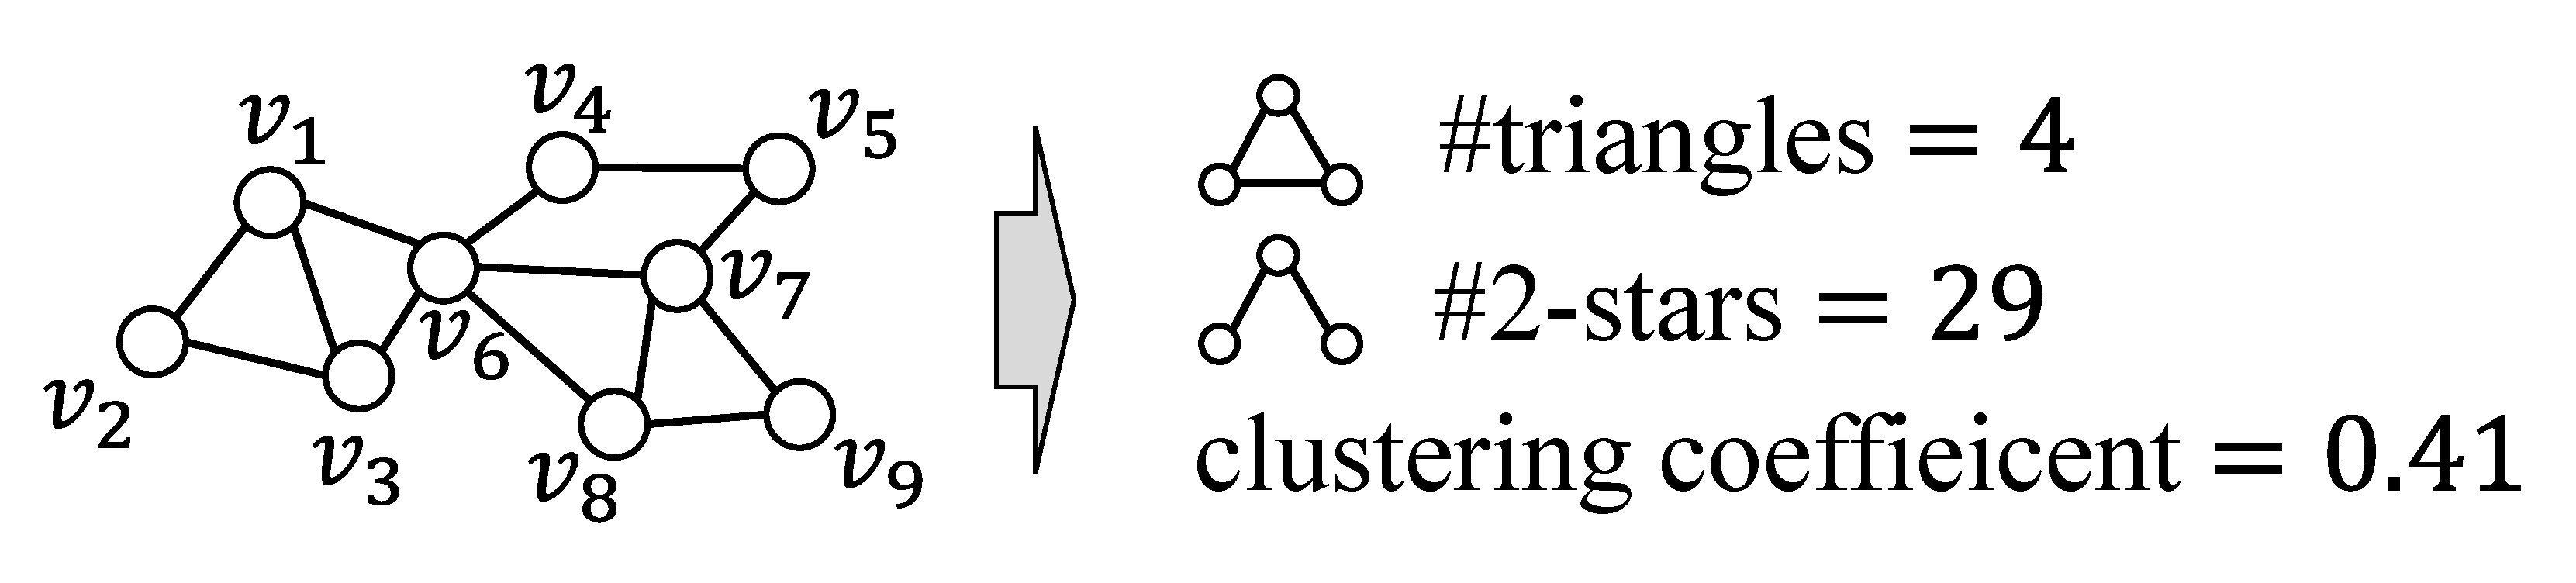
\includegraphics[width=0.85\linewidth]{fig/triangles_stars.pdf}
  
  \caption{Triangles, $2$-stars, and clustering coefficient.}
  \label{chap2-fig:triangles_stars}
\end{figure}

A recent study \cite{Imola_USENIX21} shows that the estimation error in
% triangle counting under LDP
locally private triangle counting
is significantly reduced by introducing an additional round of interaction between users and the server.
Specifically, if the server publishes the noisy graph (all noisy edges) sent by users at the first round, then each user can count her noisy triangles such that \textit{only one edge} is noisy (as she knows two edges connected to her).
Thus,
% each user
the algorithm in \cite{Imola_USENIX21} sends each user's noisy triangle count (with additional noise) to the server at the second round.
Then the server can accurately estimate the triangle count. 
% between users and the server 
% The algorithm in \cite{Imola_USENIX21} 
This algorithm also requires a much smaller number of interactions 
% between users and the server 
(i.e., only two) than collaborative approaches \cite{Kairouz_FTML21,Shokri_CCS15} that generally require many interactions. 

Unfortunately, 
% this algorithm 
the algorithm in \cite{Imola_USENIX21} 
is still
% far from practical
impractical 
for a large-scale graph.
% as shown in this paper.
Specifically, the noisy graph sent by users is dense, hence extremely large for a large-scale graph, e.g.,
$500$
% $400$
Gbits for a graph of
% about $900000$ users, as in our experiments).
a million users.
The problem is that \textit{every user} needs to download such huge data; e.g., when the download speed is $20$ Mbps (which is a recommended speed in YouTube \cite{YouTube_speed}), every user needs about 7 hours to download the noisy graph.
Since the communication ability might be limited for some users, the algorithm in \cite{Imola_USENIX21} cannot be
% applied to
used for
% a large-scale graph with diverse communication environments.
applications with large and diverse users.

In summary, existing triangle algorithms under LDP suffer from either a prohibitively large estimation error or a prohibitively 
% large 
high 
communication cost.
% For the same reason, they cannot calculate the clustering coefficient
They also suffer from the same issues when calculating the clustering coefficient.

% \colorB{
% \begin{itemize}
%     \item graph statistics; e.g., degree distribution, subgraph count (e.g., 2-stars, triangles), clustering coefficient.
%     \item privacy issue, DP, central DP, LDP.
%     \item 2-star counting under LDP is easy because...
%     \item triangle counting (hence clustering coefficient) is much harder because...
%     \item Previous work \cite{Imola_USENIX21}. Communication cost is prohibitively large (e.g., 400 Gbits for \IMDB{}).
%     \item This work
% \end{itemize}}

\smallskip
\noindent{\textbf{Our Contributions.}}~~We 
% In this work, we 
propose locally private triangle counting algorithms with a small estimation error and small communication cost.
% dramatically reduce the communication cost in accurate two-rounds triangle counting under LDP
% introduce some novel algorithms
% dramatically reduce the communication cost in locally private triangle counting
% address this issue
% by introducing some novel algorithms.
% Specifically, our contributions are:
Our contributions are as follows:

\begin{itemize}
    \item We propose two-rounds triangle algorithms
% that sample edges and then select edges each user downloads.
consisting of \textit{edge sampling} after RR and \textit{selecting edges each user downloads}.
In particular, we show that a simple extension of \cite{Imola_USENIX21} with edge sampling suffers from a large estimation error for a large or dense graph where the number of 4-cycles (such as $v_1$-$v_2$-$v_3$-$v_6$-$v_1$
% and $v_4$-$v_5$-$v_7$-$v_6$-$v_4$
in Figure~\ref{chap2-fig:triangles_stars}) is large.
To address this issue, we propose some strategies for selecting edges to download to reduce the error caused by the 4-cycles, which we call the \textit{4-cycle trick}.
\item We
show that
% the above algorithms
the algorithms with the $4$-cycle trick
still suffer from a large estimation error due to
% a large global sensitivity
% a large amount of the Laplacian noise.
large Laplacian noise for each user.
% To address this, 
To significantly reduce the Laplacian noise, 
we
propose a \textit{double clipping} technique,
which clips 
a degree (the number of edges) of each user 
% the number of edges 
with LDP and then clips the number of noisy triangles. 
% to significantly reduce the Laplacian noise.
% which significantly reduces the Laplacian noise by edge clipping and noisy triangle clipping.
% consists of edge clipping and noisy triangle clipping, to significantly reduce the global sensitivity in DP \cite{DP}.
% consisting of edge clipping and noisy triangle clipping
\item We evaluate our algorithms using two real datasets.
We show that our entire algorithms with the 4-cycle trick and double clipping
% provide the best performance, and
dramatically reduce the communication cost
% when compared with
of
\cite{Imola_USENIX21}.
For example,
% when the number of users is about $900000$,
for a graph with about $900000$ users,
we reduce the download cost from $400$ Gbits ($6$ hours when $20$ Mbps) to 
% $100$ Mbits ($5$ seconds) 
$160$ Mbits ($8$ seconds) or less 
while keeping the relative error much smaller than 1.
\end{itemize}
Thus, locally private triangle counting is now much more practical. 
% Note that the number of interactions between users and a server in our algorithms (i.e, only two) is also much smaller than collaborative approaches that generally requires a number of interactions. 
In Appendix~\ref{chap2-sec:cluster}, we also show that we can estimate the clustering coefficient with a small estimation error and download cost. 
For example, our algorithms are useful for measuring the effectiveness of friend suggestions or social recommendations in decentralized 
social networks, 
% SNS, 
e.g., Diaspora \cite{Diaspora}, Mastodon \cite{Mastodon}. 
% We published
Our source code
% with C/C++
is available at 
\cite{TriangleLDP}. 
%\cite{ComTriLDP}.
% as open-source software.

All the proofs of our privacy and utility analysis 
% The proofs of all statements 
are given in \conference{the full version \cite{Imola_arXiv22}}\arxiv{Appendices~\ref{chap2-sec:proof_seq_comp_edge_LDP}, \ref{chap2-sec:proof_algorithms}, and \ref{chap2-sec:proof_double_clip}}.

\smallskip
\noindent{\textbf{Technical Novelty.}}~~Below we explain more about 
% also clarify 
the technical novelty of this paper. 
Although we focus on two-rounds local algorithms in the same way as \cite{Imola_USENIX21}, we introduce several new algorithmic ideas previously unknown in the literature. 

First, our 4-cycle trick is totally new. 
Although some studies focus on 4-cycle counting \cite{Bera_STACS17,Kallaugher_PODS19,Manjunath_ESA11,McGregor_PODS20}, this work is the first to use 4-cycles to improve communication efficiency. 
Second, selective download of parts of a centrally computed quantity is also new. 
This is not limited to graphs -- even in machine learning, 
% or federated learning, 
there are no such strategic download techniques previously, to our knowledge. 
Third, our utility analysis of our 
% two-rounds 
triangle 
algorithms (Theorem~\ref{chap2-thm:l2loss_algorithms}) is 
% also now because it 
different from \cite{Imola_USENIX21} in that ours introduces subgraphs such as 4-cycles and $k$-stars. 
This leads us to our 4-cycle trick. 
Fourth, we propose two triangle algorithms that introduce the 4-cycle trick and show that the more tricky one provides the best performance because of 
its low sensitivity in DP.
% small Laplacian noise. 

% Fourth, 
Finally, 
our double clipping is new. 
Andrew \textit{et al.} \cite{Andrew_NeurIPS21} propose an adaptive clipping technique, which applies clipping twice. 
However, they focus on federated averaging, 
% or SGD (Stochastic Gradient Descent), 
and their problem setting is different from our graph setting. 
In particular, they require a private quantile of the norm distribution. 
In contrast, we need only a much simpler estimate: a private degree. 
Here, we use the fact that the degree has a small sensitivity (sensitivity $=1$) in DP for edges. 
We also provide a new, reasonably tight bound on the probability that the noisy triangle count exceeds a clipping threshold (Theorem~\ref{chap2-thm:triangle_excess}). 
Thanks to the two differences, we obtain a significant communication improvement: two or three orders of magnitude. 

% Finally, we show an interesting finding when we combine the 4-cycle trick and double clipping. 
% Specifically, we propose two triangle algorithms that introduce the 4-cycle trick and show that the more tricky one provides the best performance because of its low sensitivity.
